\documentclass[12pt]{book}
\let\cleardoublepage\clearpage
\usepackage[utf8]{inputenc}
\usepackage{lmodern}
\usepackage[spanish,es-tabla]{babel}
\usepackage{amsmath}
\usepackage{amsfonts}
\usepackage{amssymb}
\usepackage{color}
\usepackage{textcomp}
\usepackage[T1]{fontenc}
\usepackage{graphicx}
\usepackage{makeidx}
\makeindex
\usepackage{anysize}
\usepackage{anyfontsize}
\usepackage{pdfpages}
\usepackage[x11names,table]{xcolor}
\usepackage{tikz}
\usepackage{tcolorbox}
\usepackage[hidelinks]{hyperref}
\usepackage{caption}
\usepackage{listings}
\usepackage[left=2cm,top=2cm,right=2cm,bottom=2cm]{geometry}
\setlength{\parindent}{0cm}
\tcbset{colback=green!5!white, colframe=gray!10!black, coltitle=green!20!black, 
fonttitle=\bfseries, colbacktitle=white, coltext=gray!30!black}
\usepackage{epigraph}
\usepackage[printwatermark]{xwatermark}
\usepackage{xcolor}
\newwatermark[allpages,color=gray!10,angle=45,scale=3,xpos=0,ypos=0]{Borrador}

% Colores
\definecolor{verdep}{rgb}{0.5,0.5,0.9}
\definecolor{ccap}{rgb}{0.2,0.2,0.2}
\definecolor{csec}{rgb}{0.4,0.4,0.4}
\definecolor{csubsec}{rgb}{0.6,0.6,0.6}
\definecolor{cenun}{rgb}{0.2,0.2,0.3}
\definecolor{csol}{rgb}{0.2,0.8,0.1}
\definecolor{backcode}{rgb}{0.95,0.95,0.99}
\definecolor{dkgreen}{rgb}{0,0.6,0}
\definecolor{gray}{rgb}{0.5,0.5,0.5}
\definecolor{mauve}{rgb}{0.58,0,0.82}

% Nuevos comandos

\usepackage{titlesec}%--
\newcommand{\hsp}{\hspace{5pt}}
\titleformat{\chapter}[hang]{\huge\bfseries\color{ccap}}
{\hsp{\fontsize{35}{5}\selectfont\thechapter .}\hsp%
\hsp{\fontsize{35}{5}\selectfont}}{5pt}{\huge\bfseries}

\titleformat{\section}[hang]{\normalfont\color{csec}}%
{\filright\large\enspace\thesection\enspace}%
{8pt}{\large\bfseries\filright}%

\titleformat{\subsection}[hang]{\normalfont\color{csec}}%
{\filright\large\enspace\thesubsection\enspace}%
{8pt}{\large\bfseries\filright}%

\newcommand{\enunciado}[1]{{\it \textcolor{cenun}{#1}}\vspace{10pt}}
\newcommand{\sol}{{\textcolor{csol}{Solución.}}\vspace{10pt}}

% Code

\lstnewenvironment{matlab}{\lstset{frame=none,
  backgroundcolor=\color{backcode},
  language=Matlab,
  aboveskip=3mm,
  belowskip=3mm,
  showstringspaces=false,
  columns=flexible,
  basicstyle={\small\ttfamily},
  numbers=none,
  numberstyle=\tiny\color{gray},
  keywordstyle=\color{blue},
  commentstyle=\color{dkgreen},
  stringstyle=\color{mauve},
  breaklines=true,
  breakatwhitespace=true,
  tabsize=3,
  extendedchars=true,
  inputencoding=utf8,
  literate=%
  {°}{{\,\,$^\circ$\,\,}}1
  {á}{{\'a}}1
  {é}{{\'e}}1
  {í}{{\'i}}1
  {ó}{{\'o}}1
  {ú}{{\'u}}1
  {Á}{{\'A}}1
  {É}{{\'E}}1
  {Í}{{\'I}}1
  {Ó}{{\'O}}1
  {Ú}{{\'U}}1
}}{}

\author{Pedro Jorge De Los Santos}
\title{Ejercicios resueltos de programación en MATLAB}

\begin{document}
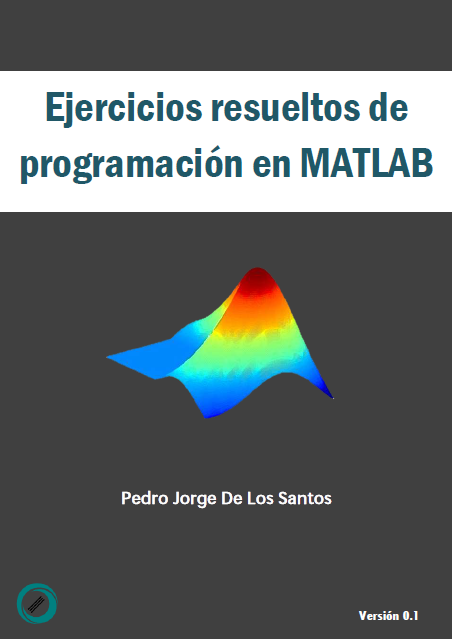
\includepdf{src/portada}
\maketitle
\tableofcontents

% Contenido

% Programación básica
% Matrices y vectores
% Cadenas de caracteres
% Gráficas
% Matemáticas
% GUIs
% POO

\chapter*{Acerca de...}

Este pequeño \textit{libro} se ha escrito con la finalidad de aportar una herramienta auxiliar a la comunidad 
hispanohablante de MATLAB. Orientado, sobre todo, a quienes dan los primeros pasos en la programación 
con este entorno de desarrollo.\\

Los problemas se han clasificado en diversas temáticas, para facilitar el estudio de los mismos. 
Todos los códigos de este libro están disponibles en el siguiente repositorio de GitHub: 
\href{https://github.com/JorgeDeLosSantos}{\bfseries\color{mauve} ERPM}.\\

El autor agradece cualquier tipo de comentario, observación u opinión, y puede remitirla 
a la dirección de correo electrónico que se adjunta posteriormente, o bien, contactándonos 
a través de las diversas plataformas cuyos enlaces se incluyen en la parte inferior.\\ \\

\texttt{Pedro Jorge De Los Santos}\\
\texttt{delossantosmfq@gmail.com}\\

\href{https://labdls.blogspot.mx}{
\includegraphics[scale=0.1]{src/blogger_logo.png}}
\href{https://www.youtube.com/user/lab2dls}{
\includegraphics[scale=0.1]{src/youtube_logo.png}}
\href{https://github.com/JorgeDeLosSantos}{
\includegraphics[scale=0.08]{src/github_logo.png}}
\href{https://www.linkedin.com/in/pjdlsl}{
\includegraphics[scale=0.1]{src/linkedin_logo.png}}
\href{https://plus.google.com/u/0/+pjdelossantos}{
\includegraphics[scale=0.1]{src/google_logo.png}}
\chapter{Programación básica e intermedia}

\section{Número par / impar}

\enunciado{Desarrolle un programa que determine si un número es par o impar.}

\sol

Este ejercicio es uno de los más comunes en los cursos básicos de programación. 
Para resolverlo hay que tener en cuenta algunas nociones básicas de matemáticas: es 
sabido que cualquier número par es divisible por 2, lo cual nos lleva al supuesto de que 
si un número es par necesariamente el resto de la división entre 2 debe ser igual a cero. 
La función rem de MATLAB devuelve 0 si el residuo de la división entera es nulo, y devuelve 1 
si es una cantidad igual o mayor a la unidad. Basándonos en lo anterior podemos diseñar 
un programa que ejecuta la comprobación y que muestre en pantalla si el número es par o impar.

\begin{matlab}
num=input('Numero: ');
if rem(num,2)==0
    disp('Numero par');
else
    disp('Numero impar');
end
\end{matlab}

El programa anterior utiliza la sentencia compuesta if-else para llevar a cabo dicha tarea. 
Es posible también usar la sentencia switch tal como se muestra enseguida, los resultados, desde luego, son iguales.

\begin{matlab}
num=input('Numero: ');
switch rem(num,2)
    case 0
        disp('Numero par');
    otherwise
        disp('Numero impar');
end
\end{matlab}

% ------------------------------------------------------------------------------------------------

\section{Lista de números pares}

\enunciado{Desarrolle un programa que proporcione los primeros números pares que se indiquen:}

\sol

Para desarrollar la solución a este problema se hará uso del operador {\it dos puntos}, el cual 
permite crear una lista o vector de valores numéricos con un cierto patrón, con la sintaxis:

\begin{verbatim}
v=a:h:b;
\end{verbatim}

Donde a es el valor inicial, h el incremento y b el valor final. En este caso necesitamos una lista 
de valores que comienze con el primer número par (2), con incrementos de 2, y cuyo valor final dependa 
de la cantidad de número pares requeridos. Por ejemplo, si se requieren 3 números pares, se esperaría que 
el último valor sea 6, que es equivalente a tener 2x3, así, de forma generalizada, el valor final será 
2n, donde n es la cantidad de números pares.

\begin{matlab}
n=input('¿Cuantos numeros pares necesita? ');
pares=2:2:2*n;
disp(pares);
\end{matlab}

% ----------------------------------------------------------------------------------------------------------

\section{Números primos} 

\enunciado{Escriba una función que le permita determinar si un número entero pasado como argumento 
es primo, en caso de serlo devolverá un valor lógico {\tt true} y un valor {\tt false} en caso contrario. 
(La función {\tt isprime} de MATLAB realiza la misma operación).}

\sol

Primero, sin tantos formalismos, un número primo es aquel cuyos únicos divisores son el uno y él mismo. 
Así, un programa básico puede estructurarse haciendo la comprobación, uno a uno, si cada número en el intervalo 
$[1, n]$ es divisor del número en cuestión. Si la cantidad de divisores es mayor a 2, entonces el número 
no es primo. Véase el código siguiente propuesto como solución:

\begin{matlab}
function r = esprimo(n)
L=1:n;
if nnz(rem(n,L)==0)==2
    r=true;
else
    r=false;
end
end
\end{matlab}

En resúmen: sea define un vector $L$ de $n$ elementos que contiene todos los números en el intervalo $[1,n]$, 
enseguida se aplica la función {\tt rem} a todos los elementos del vector $L$ y a esto se aplica la condición 
de ser igual a cero, resultando un vector de tipo lógico, donde los unos corresponden a aquellos números donde 
el residuo de la división entera es cero y por tanto divisores de $n$; finalmente, mediante la función 
{\tt nnz} se {\it cuentan} los elementos que no son ceros, si estos son igual a dos, entonces se tiene un 
número primo.

% -------------------------------------------------------------------------------------------------------

\section{Área y perímetro de un círculo}

\enunciado{Escriba un programa cuya entrada sea el radio del círculo e imprima el valor del área y 
perímetro correspondiente.}

\sol

Para resolver este problema, lo primero es remitirnos a los cursos de geometría básica y recordar 
que el área y perímetro (circunferencia) de un círculo vienen dados por:

$$A=\pi r^2$$
$$P=2 \pi r$$

Con lo anterior se plantea una solución:

\begin{matlab}
radio=input('Radio del círculo: ');
area=pi*radio^2;
perimetro=2*pi*radio;
fprintf('Área: %g \n',area);
fprintf('Perímetro: %g \n',perimetro);
\end{matlab}

% ============================================================================================================

\section{Conversión grados – radianes}

\enunciado{Utilice cualquier sentencia de selección múltiple para desarrollar un programa que le permita hacer la conversión de grados sexagesimales a radianes y viceversa.}

\sol

Sea $\theta_r$ un ángulo dado en radianes y $\theta_g$ en grados sexagesimales, las {\it formulas} de 
conversión resultan en:

$$\theta_r = \theta_g \left(\frac{\pi}{180}\right)$$
$$\theta_g = \theta_r \left(\frac{180}{\pi}\right)$$

\begin{matlab}
opcion=input(['Seleccione una opción: \n 1. Grados a radianes'...
'\n 2. Radianes a grados \n']);
theta=input('Inserte la magnitud del angulo: ');
switch opcion
    case 1
        thetaR=theta*pi/180;
        fprintf('%g ° = %g rad \n',theta,thetaR);
    case 2
        thetaG=theta*180/pi;
        fprintf('%g rad = %g ° \n',theta,thetaG);
    otherwise
        disp('Opcion incorrecta');
end
\end{matlab}


% ============================================================================================================
\section{Promedio de una lista de valores}

\enunciado{Realice un programa que pida la cantidad de elementos o datos a introducir y que posteriormente sean ingresados manualmente, con los datos anteriores calcular el promedio de los mismos.}

\sol

\begin{matlab}
n=input('Cantidad de datos a introducir: ');
for i=1:n
    D(i)=input(['Dato ',num2str(i),': ']);
end
fprintf('El promedio de los datos introducidos es %g\n',mean(D));
\end{matlab}


% ============================================================================================================
\section{Sucesión de Fibonacci}

\enunciado{Escriba un programa que imprima en pantalla los primeros n términos de la sucesión de Fibonacci.}

\sol

La sucesión de Fibonacci es una sucesión infinita de números naturales, cuyos términos resultan de la 
suma de los dos términos anteriores. Los primeros dos términos son 1 y 1, y enseguida el resto siguen 
el patrón descrito con anterioridad, así, algunos de los primeros términos se muestran enseguida:

$$ 1,1,2,3,5,8,13,21,34,55,... $$

Luego, cada término de la sucesión se calcula bajo la siguiente especificación: $f_i=f_{i-1}+f_{i-2}$. 
La implementación en MATLAB resulta muy sencilla, se definen inicialmente los dos primeros términos y 
enseguida se concatenan los valores de la sucesión que siguen el patrón mencionado, mediante un bucle. 
Un código de ejemplo se muestra a continuación:

\begin{matlab}
n=input('Numero de terminos a mostrar: ');
F=[1 1];
for i=3:n
    F(i)=F(i-1)+F(i-2);
end
disp(F);
\end{matlab}


% ============================================================================================================
\section{Múltiplos de un número}

\enunciado{Desarrolle una función que devuelva los primeros k múltiplos de un determinado número.}

\sol

Un múltiplo de un número es aquel que lo contiene un número entero de veces. Luego, los primeros $k$ 
múltiplos de un número $N$ cualesquiera, vienen dado por $<1,2,...,k-1,k>*N$. La implementación 
en MATLAB es muy sencilla, utilizando la notación de dos puntos para crear un vector cuyos elementos 
sean los enteros desde 1 hasta $k$.

\begin{matlab}
function x = multiplos(num,k)
% Devuelve los primeros k multiplos de num.
%
x=(1:k)*num;
end
\end{matlab}


% ============================================================================================================
\section{Ecuación cuadrática}

\enunciado{Escriba una función que le permita resolver una ecuación de segundo grado de la forma 
$ax^2+bx+c=0$, siendo los coeficientes los argumentos de entrada y las raíces de la ecuación los valores de salida.}

\sol

La solución general de una ecuación de segundo grado de la forma $ax^2+bx+c=0$ viene dada por la tan conocida 
{\bf formula general}.

$$x_{1,2}=\frac{-b\pm\sqrt{b^2-4ac}}{2a}$$

\begin{matlab}
function [x1,x2]=ecuadratica(a,b,c)
% Resuelve una ecuacion de segundo orden, siendo
% los argumentos de entrada los coeficientes de
% la misma.
x1=(-b+sqrt(b^2-4*a*c))/(2*a);
x2=(-b-sqrt(b^2-4*a*c))/(2*a);
end
\end{matlab}


\section{Tiempo de vida}

\enunciado{Desarrolle un script que le permita calcular el número de años, meses, días y horas que ha vivido un individuo.}

\sol

\begin{matlab}
D=input('Día de nacimiento: ');
M=input('Mes de nacimiento: ');
A=input('Anio de nacimiento: ');
actual=now;
nac=datenum(A,M,D);
fprintf('\n¿Cuanto has vivido?\n');
fprintf('Anios = %g \n',(actual-nac)/365);
fprintf('Meses = %g \n',(actual-nac)/30);
fprintf('Dias = %g \n',(actual-nac));
fprintf('Horas = %g \n',(actual-nac)*24);
\end{matlab}


% =========================================================================================================
\section{Adivinar el número}

\enunciado{Escriba un programa que genere un número entero aleatorio entre 1 y 100, y posteriormente le pida al usuario tratar de adivinar el número en cuestión, para cada intento el programa debe mostrar si el número que se trata de adivinar es mayor o menor al propuesto por el jugador. El programa termina cuando el jugador adivina el número, imprimiéndose en pantalla la cantidad de intentos realizados.}

\sol

Para generar el número entero aleatorio en el rango $[1,100]$ se utilizará la función \texttt{randi}, que devuelve un 
entero aleatorio en el intervalo que se especifique. Dentro de un bucle while se hacen las comprobaciones de equivalencia 
del número aleatorio con el número propuesto por el jugador. Además se utiliza un contador que se incrementa en la unidad 
cada vez que se ejecuta un ciclo. El ciclo se \textit{rompe} cuando el jugador adivina el número mediante la 
instrucción \texttt{break}.

\begin{matlab}
n=randi([1 100]);
k=0;
while 1
    np=input('¿Numero?: ');
    k=k+1;
    if n<np
        disp('Es menor');
    elseif n>np
        disp('Es mayor');
    else
        break;
    end
end
fprintf('Lo has conseguido en %g intentos \n',k);
\end{matlab}

% =========================================================================================================
\section{Imprimir rombo} 

\enunciado{Desarrolle un programa que imprima un rombo de asteriscos en pantalla para un valor 
dado de n, donde n es el número de filas y/o columnas totales del rombo, debe notar que n será 
siempre un entero impar mayor o igual 3. Para una mejor comprensión se muestran a continuación 
los resultados para n=3 y n=7.}

\begin{center}
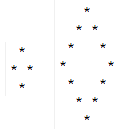
\includegraphics[scale=1]{src/rombo.png}
\end{center}

\sol

\begin{matlab}
n=input('Numero de filas del rombo: ');
R='';
for i=1:n
    if i<=ceil(n/2)
        R(i,[ceil(n/2)+(1-i) ceil(n/2)+(i-1)])='*';
    else
        R(i,[ceil(n/2)-(n-i) ceil(n/2)+(n-i)])='*';
    end
end
disp(R);
\end{matlab}

\section{Factorial de un número}

\enunciado{El factorial de un entero positivo n viene dado por $n!=(1)(2)...(n-1)(n)$, es decir, el producto 
de todos los enteros desde 1 hasta n. Realice un programa que devuelva el factorial de un número 
introducido (Recuerde que por definición el factorial de 0 es igual a la unidad).}

\sol

\begin{matlab}
N=input('Introduzca un numero entero: ');
k=1;
fact=1;
while k<=N
    fact=k*fact;
    k=k+1;
end
fprintf('\n %d! = %d\n\n',N,fact);
\end{matlab}


\section{Imprimir triángulo}

\enunciado{Realice un script que imprima en pantalla un triángulo de asteriscos, el programa debe tener como entrada el número de filas del triángulo.}

\sol

\begin{matlab}
n=input('Numero de filas: ');
A='';
for i=1:n
    A(i,1:2:2*i)='*';
end
disp(A)
\end{matlab}


\section{Sumatoria de n múltiplos de 5}

\enunciado{Escriba un programa que devuelva la suma de los primeros n múltiplos de 5, que además cumplan la condición de no ser múltiplos de 10.}

\begin{matlab}
N=input('Multiplos a sumar: ');
suma=0;
mult=5;
k=0;
while k<N
    if rem(mult,10)
        suma=suma+mult;
        k=k+1;
    end
    mult=mult+5;
end
disp(suma);
\end{matlab}

\section{Tabla de funciones trigonométricas}

\enunciado{Desarrolle un programa que imprima una tabla de valores para las funciones trigonométricas más comunes en el rango 0° a 45° (seno, coseno y tangente).}

\begin{matlab}
fprintf('====================================\n');
fprintf('°    sin(x)      cos(x)      tan(x)\n');
fprintf('====================================\n');
for x=0:pi/180:pi/4
    fprintf('%0.0f \t %0.4f \t %0.4f \t %0.4f\n',...
        x*(180/pi),sin(x),cos(x),tan(x));
end
\end{matlab}

\section{Tabla de multiplicar} 

\enunciado{Escriba un programa que pida al usuario un entero positivo del cual se desarrollará e imprimirá en pantalla su tabla de multiplicación del 1 al 10, por ejemplo:}

\begin{center}
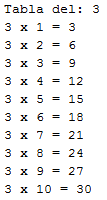
\includegraphics[scale=0.8]{src/tablamult.png}
\end{center}

\sol

\begin{matlab}
N = input('Tabla del: ');
for k = 1:10
    fprintf('%g x %g = %g\n',N,k,N*k);
end
\end{matlab}
\chapter{Matrices y vectores}

\section{Valor máximo de un vector}

\enunciado{MATLAB utiliza la función max para determinar el máximo valor de un vector, escriba un programa 
que lleve a cabo la misma tarea, evitando hacer uso de la función max}.

\sol

Existen, claro, múltiples formas de proceder para resolver este problema, por ejemplo, se podrían 
ordenar los elementos del vector en forma descendente y entonces tomar el primer elemento que 
correspondería al de mayor valor. Pero, para este caso vamos a proceder de la forma más \textit{simplista}, 
utilizando un bucle for para recorrer el vector e ir comprobando, elemento a elemento, si un elemento 
anterior es menor al actual. Suponemos, en principio, que el valor máximo es el primer elemento del vector 
y enseguida hacemos la comprobación para el resto de elementos, tal como se muestra.

\begin{matlab}
v=input('Vector: ');
maxv=v(1);
for i=2:length(v)
    if v(i)>maxv
        maxv=v(i);
    end
end
fprintf('El valor maximo es %g\n\n',maxv);
\end{matlab}

\section{Matriz identidad}

\enunciado{La función eye crea una matriz identidad; programe una función llamada idmat que reciba 
como argumento la dimensión de la matriz (cuadrada) y devuelva una matriz identidad.}

\sol

\begin{matlab}
function M = idmat(n)
M(1:n,1:n)=0;
for i=1:n
    M(i,i)=1;
end
end
\end{matlab}


\section{Elementos diferentes en un vector}

\enunciado{Escriba un programa que determine el número de elementos diferentes en un vector.}

\sol

\begin{matlab}
v=input('Vector: ');
v=sort(v);
k=1;
for i=2:length(v)
    if v(i)~=v(i-1)
        k=k+1;
    end
end
fprintf('Hay %d elementos diferentes\n\n',k);
\end{matlab}

\section{Ordenar elementos de un vector}

\enunciado{La función sort de MATLAB ordena los elementos de un vector en forma ascendente o descendente, escriba una función llamada ordenarasc cuyo argumento de entrada sea un vector y devuelva como salida el mismo vector ordenado en forma ascendente (de menor a mayor).}

\sol

\begin{matlab}
function xo = ordenarasc(x)
% Ordena un vector en forma ascendente
%
xo=zeros(size(x));
i=1;
while i<=length(xo)
    ne=length(x(x==min(x)));
    xo(i:i+ne-1)=min(x);
    x(x==xo(i))=[];
    i=i+ne;
end
end
\end{matlab}

\section{Adjunta de una matriz de 3x3}

\enunciado{Desarrolle una función que reciba como parámetro de entrada una matriz de 3x3 y que devuelva como salida la adjunta de dicha matriz.}

\sol

\begin{matlab}
function X = adjunta3(A)
% Calcula la adjunta de una matriz de 3x3
% Entrada:
%         A   -   Matriz de 3x3
% Salida:
%         X   -   Matriz adjunta de A
%
if size(A,1)~=3 || size(A,2)~=3
    error('Introduzca una matriz de 3x3');
end
MC=zeros(size(A));
idx=1:3;
for i=1:size(A,1)
    for j=1:size(A,2)
        idxf=idx(idx~=i);
        idxc=idx(idx~=j);
        cof=A(idxf,idxc);
        if rem(i+j,2)
            MC(i,j)=-det(cof);
        else
            MC(i,j)=det(cof);
        end
    end
end
X=MC';
end
\end{matlab}


\section{Inversa de una matriz 2x2}

\enunciado{Desarrolle una función llamada \texttt{inversa22} que calcule la inversa de una matriz de 2x2. Evite usar 
la función \texttt{inv} de MATLAB.}

\sol

Una matriz de 2x2 tiene la forma general:

$$
A=\left[
\begin{array}{cc}
a & b \\
c & d \\
\end{array}
\right]
$$

Del álgebra lineal sabemos que la inversa de una matriz de esta forma viene dada por:

$$
A^{-1}=\frac{1}{det(A)}
\left[
\begin{array}{cc}
d & -c \\
-b & a \\
\end{array}
\right] = 
\frac{1}{ad-bc}
\left[ \begin{array}{cc}
d & -c \\
-b & a \\
\end{array} \right]
$$

Implementando lo anterior en MATLAB:


\chapter{Cadenas de caracteres}

\section{Invertir una cadena de texto}

\enunciado{Escriba un programa que le permita invertir una palabra ingresada, por ejemplo, si usted 
introduce MATLAB deberá devolverle BALTAM.}

\sol

En esencia lo que se debe hacer es \textit{invertir} los indices del vector tipo char en 
el cual se guarda la cadena de texto.

\begin{matlab}
cad=input('Introduzca una palabra: ','s');
disp(cad((end:-1:1)));
\end{matlab}

\section{Contar palabras}

\enunciado{Desarrolle un script que reciba como entrada una cadena de caracteres y que devuelva 
la cantidad de palabras que la componen. Para este caso se asumirá que el texto pasado como dato 
de entrada tiene una estructura coherente y libre de cualquier secuencia extraña de signos de 
puntuación u otro tipo de caracteres diferentes a los alfanuméricos.}

\sol

\begin{matlab}
txt = input('Inserte un texto: ','s');
resto = txt;
k = 0; % Inicializa contador
while true
   [palabra, resto] = strtok(resto, ' ');
   if isempty(palabra),  break;  end
   k = k + 1;
end
fprintf('No. de palabras encontradas: %d\n\n',k);
\end{matlab}


\section{Contar vocales en una cadena de texto}

\enunciado{Escriba un programa que reciba como entrada una frase o cadena de texto y que muestre como salida el número de vocales que contiene dicha frase.}

\sol

\begin{matlab}
cad=input('Introduzca una cadena de texto: ','s');
k=0;
for i=1:length(cad)
    switch cad(i)
        case {'A','a','E','e','I','i','O','o','U','u'}
            k=k+1;
        otherwise
            % ...
    end
end
fprintf('Numero de vocales: %g\n\n',k);
\end{matlab}


\section{Ordenar palabras}

\enunciado{Escriba un programa que ordene las palabras contenidas en una cadena de caracteres, imprimiéndolas en pantalla.}

\sol



\section{Cifrado básico}

\enunciado{El método de cifrado más simple es el cifrado por desplazamiento, que consiste en remplazar un caracter 
por otro ubicado {\bf n} posiciones a la derecha en la tabla de código ASCII. Por ejemplo, si tenemos la palabra 
{\bf perro}, y queremos cifrarla desplazando tres lugares obtendríamos: {\bf shuur}. En la figura siguiente se muestra 
un esquema de lo anterior.}

\begin{center}
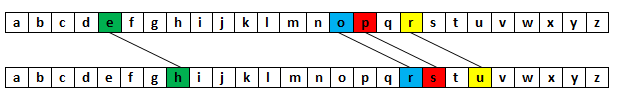
\includegraphics[scale=0.8]{src/cifrado.png}
\end{center}

\enunciado{Desarrolle un programa que tenga como entrada una cadena de caracteres y devuelva en pantalla 
la cadena cifrada mediante el desplazamiento por tres posiciones.}



\chapter{Gráficas}

\section{Gráfica de una función a trozos}

\enunciado{Escriba un programa que grafique la siguiente función a trozos:}

$$\[f(x)=\left\{ 
\begin{array}{cc}
\sin (x) & x<-\pi   \\
x+2 & -\pi \le x\le 2  \\
-x+3 & x>2  \\
\end{array} \right.\]$$

\begin{matlab}
x=-10:0.01:10;
y1=sin(x(x<-pi));
y2=x(x>=-pi & x<=2)+2;
y3=-(x(x>2))+3;
plot(x,[y1 y2 y3],'linewidth',2);
\end{matlab}

\begin{center}
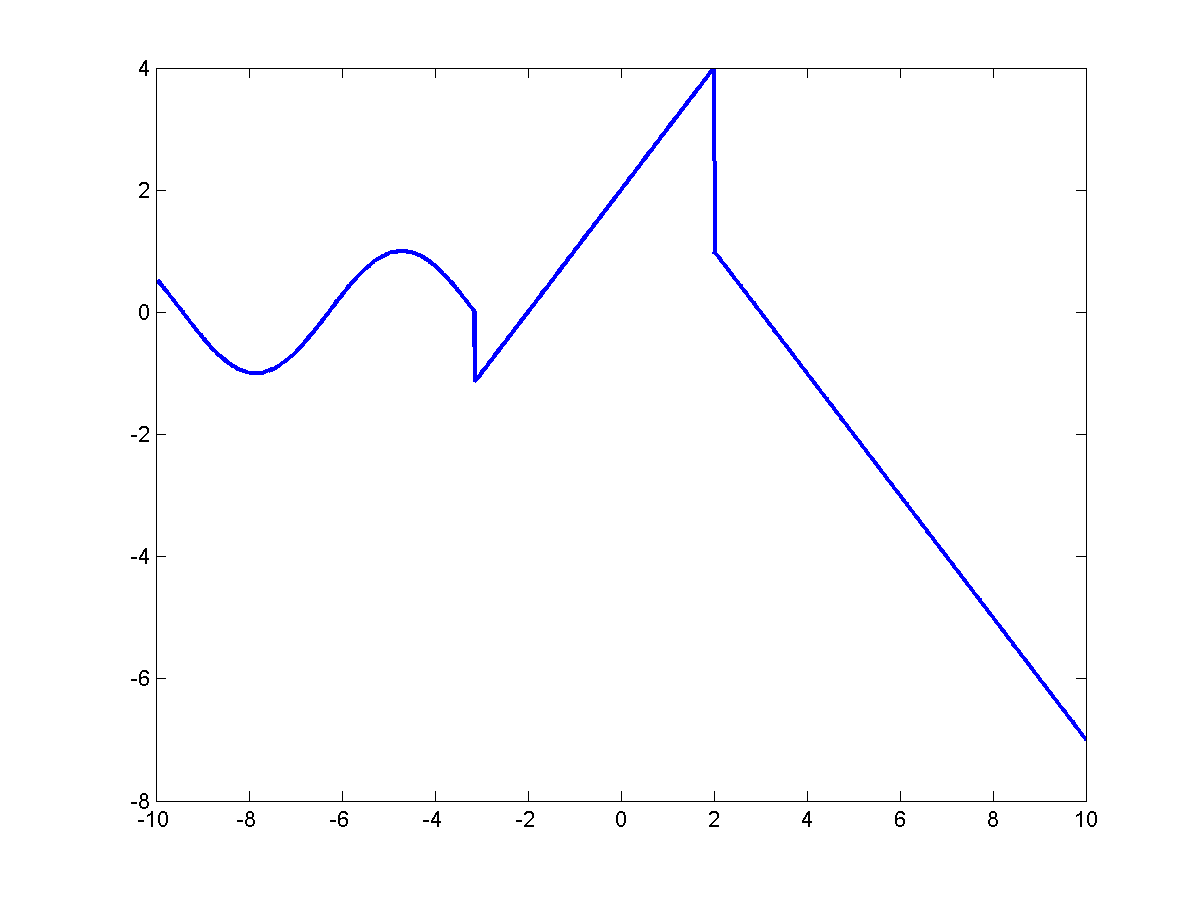
\includegraphics[scale=0.7]{src/graf_trozos.png}
\end{center}

\section{Gráfica de una desigualdad (inecuación)}

\enunciado{MATLAB no proporciona de manera nativa una función para trazar gráficas de inecuaciones, 
por ello el objetivo de este ejercicio es desarrollar una función llamada inecgraf, cuyos argumentos 
de entrada sean: la inecuación dada como una cadena de caracteres y el intervalo en el cual se 
graficará (vector de dos elementos).}

\sol

\begin{matlab}
function inecgraf(I,R)
% Grafica una desigualdad (inecuacion) en un rango
% especificado.
%
% Argumentos de entrada:
%            I    -   Inecuacion
%            R    -   Rango en el cual se trazara la
%                     grafica.
%

set(gca,'NextPlot','add'); 
axis([R(1) R(2) R(1) R(2)]);
dd=(R(2)-R(1))/50;
[x,y]=meshgrid(R(1):dd:R(2));
[f,c]=find(eval(I));
h=zeros(1,length(f));
for i=1:length(f)
        h(i)=plot(x(f(i),c(i)),y(f(i),c(i)),'b*','MarkerSize',2);
end
end
\end{matlab}

\section{Gráfica de una esfera}

\enunciado{Desarrolle una función \texttt{esfera} cuyos parámetros de entrada sean: el radio, y las coordenadas $x,y,z$ 
del centro. Con los datos anteriores trace una esfera, apoyándose en la función \texttt{sphere} nativa de MATLAB.}

\sol


\chapter{Matemáticas}

\section{Ecuación de la recta que pasa por dos puntos}

\enunciado{Desarrolle un programa cuyos valores de entrada sean las coordenadas $(x_1,y_1)$  y $(x_2,y_2)$  
de dos puntos y que devuelva en pantalla la ecuación de la recta que pasa por estos puntos.}

\begin{matlab}
x1=input('x1: ');
y1=input('y1: ');
x2=input('x2: ');
y2=input('y2: ');
m=(y2-y1)/(x2-x1);
b=(-x1*m)+y1;
if b<0
    signo='- ';
elseif b>0 
    signo='+ ';
else
    signo='';
    b='';
end 
if m==1
    m='';
end
y=['y = ',num2str(m),' x ',signo,num2str(abs(b))];
fprintf('\nEcuacion de la recta:  %s\n\n',y);
\end{matlab}
\chapter{Interfaces gráficas de usuario}

Comunmente se denomina interfaz gráfica de usuario (GUI) a un conjunto de objetos gráficos mostrados en una 
ventana, que el usuario de un ordenador utiliza para interactuar con el sistema operativo o el software en 
ejecución. En MATLAB las GUI normalmente incluyen botones, campos de texto, check boxes, menús desplegables, 
list boxes, tablas, entre otros que facilitan la interacción del usuario. Cada uno de estos elementos gráficos 
es programado para responder a una determinada acción realizada por el usuario.

\section{El hola mundo en GUI}

\enunciado{Desarrolle una interfaz gráfica que contenga un botón, el cual al ser presionado por el usuario deberá \textit{responder} mostrando un cuadro de dialogo (msgbox) con la clásica cadena \textit{hola mundo}.}

\sol

\begin{matlab}
function HolaMundo
figure('MenuBar','None',...
    'NumberTitle','off',...
    'Name','Hola Mundo');
 
uicontrol('style','push',...
    'String','Botón',...
    'Callback','msgbox(''Hola mundo'')');
end
\end{matlab}

\section{Ventana multicolor}

\enunciado{Programe una interfaz gráfica que no contenga control gráfico alguno, y que solamente cambie de color a cada cierto tiempo, esto hasta que el usuario cierre la ventana correspondiente.}

\sol

\begin{matlab}
function CambiaColor
f = figure('MenuBar','none',...
    'NumberTitle','off',...
    'Name','Cambia Color');
 
while ishandle(f)
    set(f,'Color',rand(1,3));
    pause(0.5);
    drawnow;
end
 
end
\end{matlab}

\section{Lista de archivos M.}

\enunciado{Desarrolle una GUI con un List Box, el cual debe contener una lista de los nombres de archivos *.m ubicados en el mismo directorio. Al presionar cada uno de los elementos de la lista debe abrir el archivo seleccionado en el editor de MATLAB.}

\sol

\begin{matlab}
function ListaArchivosM
figure('MenuBar','none',...
    'NumberTitle','off',...
    'Name','Lista Archivos',...
    'Position',[0 0 200 300]);
centerfig();
 
archivos_m = dir('*.m');
archivos_m = struct2cell(archivos_m);
uicontrol('style','listbox',...
    'String',archivos_m(1,:),...
    'Units','Normalized',...
    'Position',[0.02 0.02 0.96 0.96],...
    'Callback',@edit_call);
 
    function edit_call(src,~)
        str = get(src,'String');
        k = get(src,'Value');
        edit(str{k});
    end
end
\end{matlab}

\section{Mini Calculadora}

\enunciado{Diseñe y desarrolle una interfaz gráfica de usuario que asemeje el comportamiento de una calculadora muy sencilla. Debe contener cuatro botones correspondientes a los operadores aritméticos básicos, dos campos editables que permitan insertar los datos de entrada y otro campo estático o editable que permita mostrar el resultado de la operación realizada.}

\sol

\begin{matlab}
function MiniCalculadora
figure('MenuBar','None',...
    'NumberTitle','off',...
    'Name','Mini Calculadora',...
    'Resize','off',...
    'Position',[0 0 300 150]);
centerfig();
 
% ============================= DATOS ===============================
panel_datos = uipanel('Units','Pixels',...
    'Position',[10 50 280 95]);
 
uicontrol(panel_datos,'Style','text',...
    'String','# 1',...
    'Units','Normalized',...
    'Position',[0 0.67 0.4 0.25]);
hN1=uicontrol(panel_datos,'Style','edit',...
    'String','',...
    'Units','Normalized',...
    'Position',[0.45 0.72 0.5 0.25]);
 
uicontrol(panel_datos,'Style','text',...
    'String','# 2',...
    'Units','Normalized',...
    'Position',[0 0.33 0.4 0.25]);
hN2=uicontrol(panel_datos,'Style','edit',...
    'String','',...
    'Units','Normalized',...
    'Position',[0.45 0.38 0.5 0.25]);
 
uicontrol(panel_datos,'Style','text',...
    'String','Resultado',...
    'Units','Normalized',...
    'Position',[0 0 0.4 0.25]);
hR=uicontrol(panel_datos,'Style','edit',...
    'String','',...
    'Units','Normalized',...
    'Position',[0.45 0.05 0.5 0.25],...
    'BackG',ones(1,3)*0.8);
 
% ===================== BOTONES OPERADORES ============================
panel_botones = uipanel('Units','Pixels',...
    'Position',[10 5 280 40]);
 
OPERADORES = '+-*/';
 
for k = 1:length(OPERADORES)
    uicontrol(panel_botones,'style','push',...
        'String',OPERADORES(k),...
        'Units','normalized',...
        'Position',[(k-1)*(1/4) 0 1/4 1],...
        'FontSize',16,...
        'FontWeight','bold',...
        'Callback',@calcular);
end
 
    function calcular(src,~)
        n1 = get(hN1,'String'); % Primer número
        n2 = get(hN2,'String'); % Segundo número
        oper = get(src,'String'); % Operador
        set(hR,'String',num2str(eval([n1,oper,n2])));
    end
 
end
\end{matlab}

\section{Visor de imágenes (Nivel I)}

\enunciado{Desarrolle una GUI que funcione como un visor de imágenes simple, el cual debe contener un menú Archivo y dentro de este dos sub-menús llamados Abrir y Salir. La opción Abrir debe mostrar al usuario un explorador de archivos interactivo (uigetfile) que le permita seleccionar una imagen en formato PNG y enseguida mostrarla en un axes ubicado dentro la misma GUI (utilice las funciones imread e imshow para la manipulación de la imagen). La opción Salir, en este caso, es auto-descriptiva.}

\sol

\begin{matlab}
function AbrirImagen
f = figure('MenuBar','None',...
    'NumberTitle','off',...
    'Name','Abrir imagen');

% ====================== MENÚ ============================
hMenu = uimenu(f,'Label','Archivo');
uimenu(hMenu,'Label','Abrir','Callback',@abrir_img);
uimenu(hMenu,'Label','Salir','Callback','close(gcf)');

% ===================== AXES ============================
ax = axes('Units','Normalized',...
    'Position',[0 0 1 1],...
    'Visible','off');

    function abrir_img(~,~)
        [filename, pathname] = uigetfile('*.PNG', 'Seleccione una imagen');
        if isequal(filename,0) || isequal(pathname,0)
            return;
        else
            X = imread(fullfile(pathname,filename));
            imshow(X);
        end
    end
end
\end{matlab}
\chapter{POO}

\section{La clase Persona}

\enunciado{Defina una clase llamada Persona, cuyos atributos serán nombre y edad, mismos que serán pasados como argumento en el constructor de la clase. Además, la clase debe contener un método crecer que recibirá como argumento un entero positivo que indicará los años que \textit{crecerá} el objeto, desde luego modificando el atributo edad.}

\sol

\begin{matlab}
classdef Persona < handle
    
    properties
        nombre;
        edad;
    end
    
    methods
        function obj = Persona(nombre,edad)
            obj.nombre = nombre;
            obj.edad = edad;
        end
        
        function crecer(obj,anios)
            obj.edad = obj.edad + anios;
        end
    end
    
end
\end{matlab}


\section{Clase Math (Métodos estáticos)}

\enunciado{Desarrolle una clase Math que contenga los atributos constantes E (constante e) y PI (constante $\pi$), y los métodos estáticos sumar, multiplicar, redondear, mayor y menor.}

\sol

\begin{matlab}
classdef Math
    % Clase Math
    
    properties (Constant = true)
        % Atributos constantes
        PI = pi;
        E = exp(1);
    end
    
    methods (Static)
        % Métodos estáticos
        function r = sumar(a,b)
            r = a + b;
        end
        
        function r = multiplicar(a,b)
            r = a * b;
        end
        
        function r = redondear(n)
            r = round(n);
        end
        
        function r = mayor(a,b)
            r = a;
            if b > a
                r = b;
            end
        end
        
        function r = menor(a,b)
            r = a;
            if b < a
                r = b;
            end
        end
    end
    
end  
\end{matlab}


%\printindex

\end{document}
